\documentclass[9pt]{extarticle}

\usepackage[utf8]{inputenc}
\usepackage[T1]{fontenc}
\usepackage{lmodern}
\usepackage{graphicx}
\usepackage{color}
\usepackage{hyperref}
\usepackage{amsmath}
\usepackage{amsfonts}
\usepackage{epstopdf}
\usepackage[table]{xcolor}
\usepackage[a4paper, total={6in, 10in}]{geometry}
\usepackage{enumitem}
\usepackage[export]{adjustbox}


\graphicspath{ {./Figures/} }

\begin{document}

{\huge Andrew Sivaprakasam | Final Project - Progress Report 1}
\begin{center}
Final Project Repo: \url{https://github.com/sivaprakasaman/BME_511_FinalProject} 
\end{center}

Current State of the project:

\begin{enumerate}
\item \underline{Evaluate Stimulus Quality: } The stimuli provided from the Philharmonia database seem to be appropriate and of good quality. There are enough instruments with A4 pitch to asses timbre. I am planning to select an A4 pitch from Banjo, Clarinet, Flute, Trombone, and Violin. Consistent with previous work, the distribution of energy within the harmonics seems to contribute strongly to timbral characteristics. As for investigating articulation and expression, there are several different sounds available, but to start simple the violin \textit{martele} and \textit{spiccato} sounds may be good. More percussive instruments (i.e. tambourine) may be a better way to assess expression since they are not centered around a particular pitch (and have very clear envelope characteristics). See attached spectrograms.

\item \underline{Model Implementation/apPSTH analysis}: The BEZ2018 Model is working, and I'm able to get PSTHs for a stimulus of interest. Still playing with parameters and looking into what they do. 

\item \underline{Evaluating the Question/What metrics to use: } Still working on this. The apPSTH measures and Satya's code provide a good basis for studying ENV and TFS, but I'm still trying to quantify how well ENV and TFS are coded. I'm thinking I need to look at how highly the PSD of the ENV auditory nerve responses are correlated with the PSD of the ENV of the stimulus and  a similar metric for TFS. Or, I could see how the well the PSD of AN TFS/ENV responses to music-noise chimaeras and non-chimaeras are correlated. I'm still thinking this through. Goal is to have this a good bit more fleshed out by next week. I think the question will be more focused on timbral \textit{coding} rather than \textit{perception}, since \textit{perception} would probably require behavioral data.
\end{enumerate}

\textbf{Figures:}\\

\centering
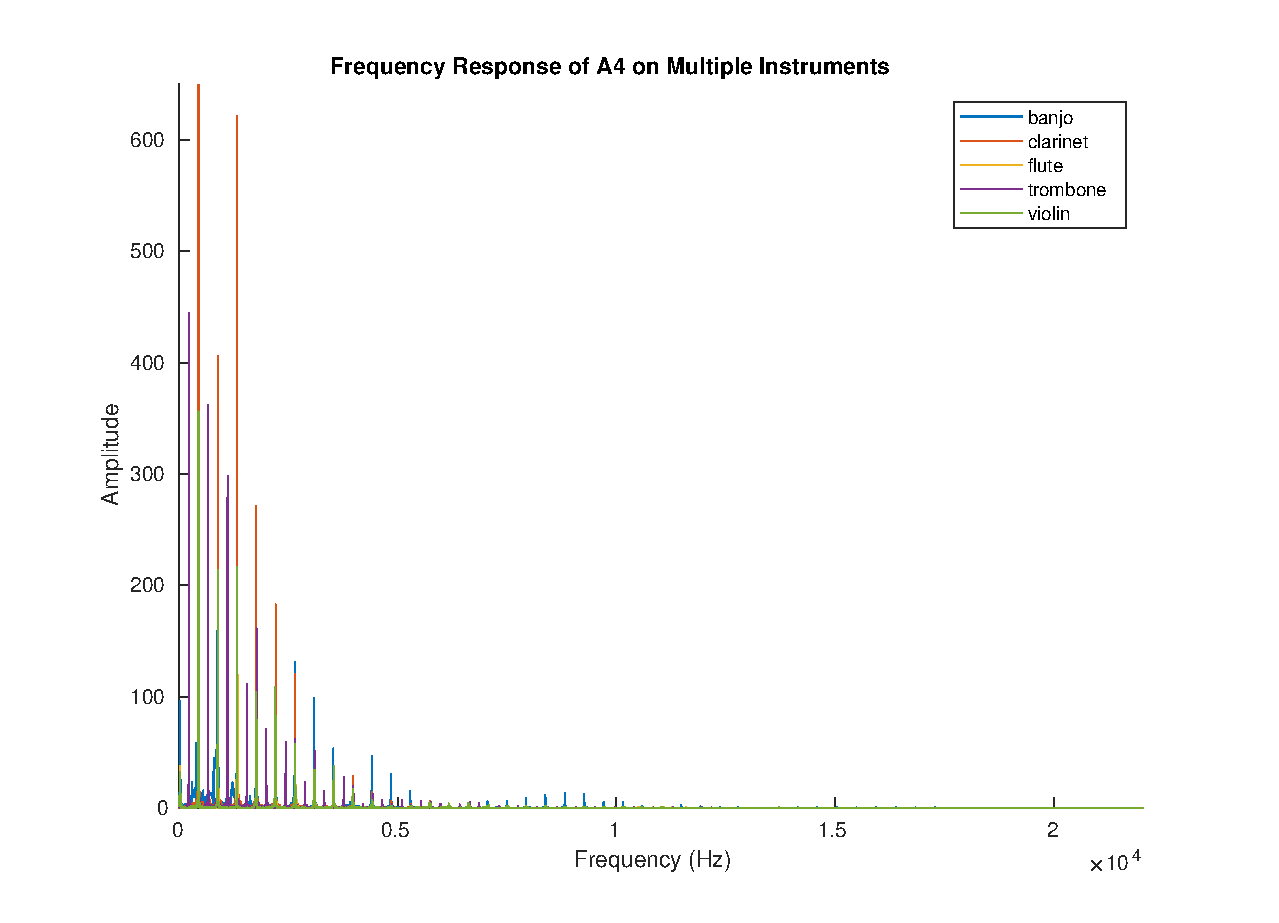
\includegraphics[width = .45\textwidth]{fft_all}\\

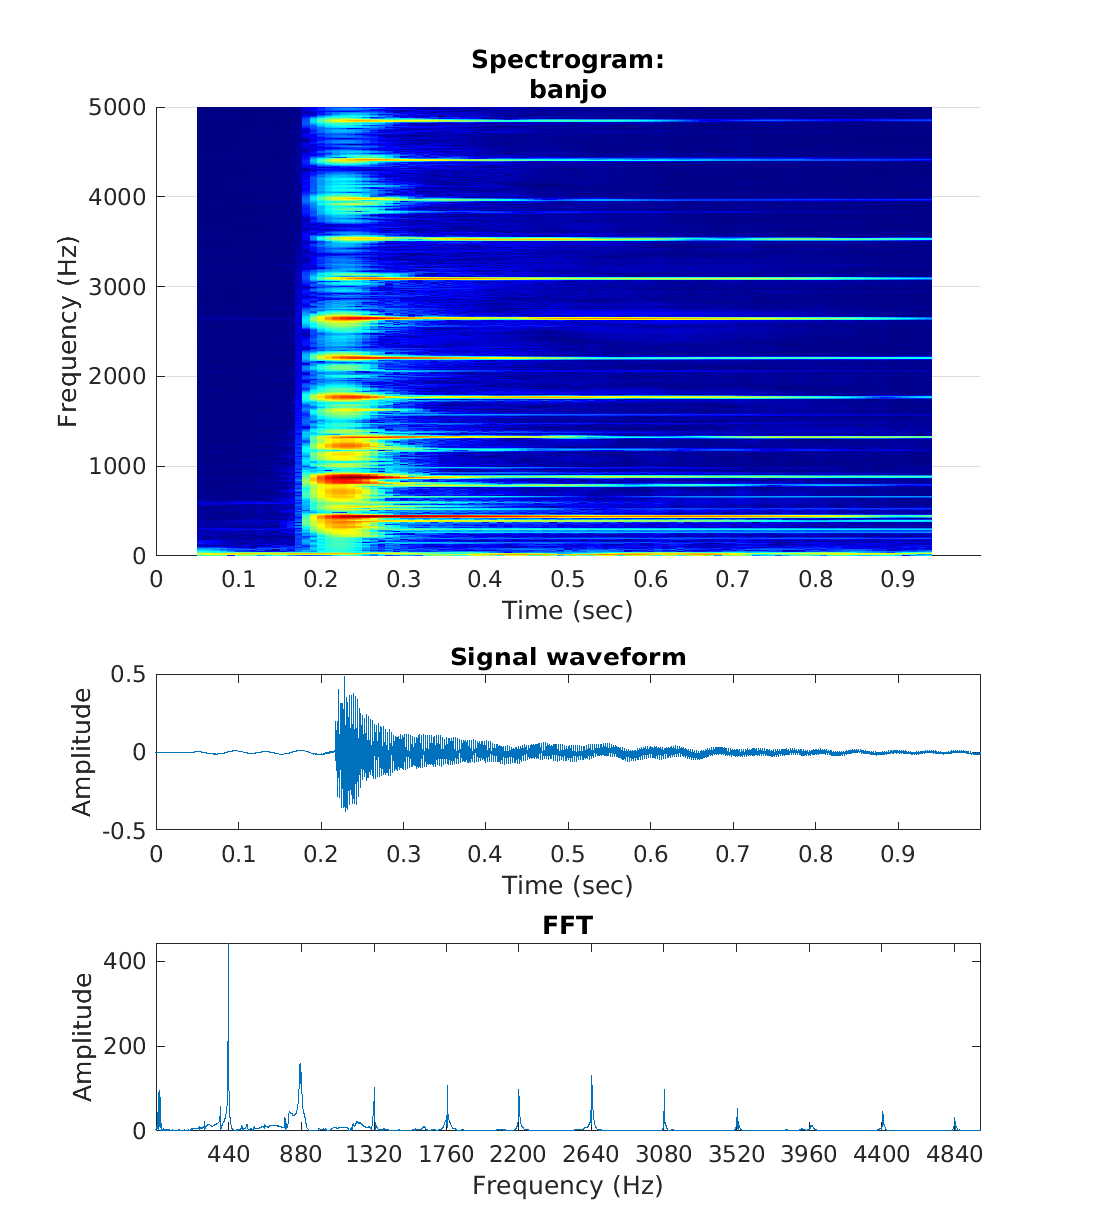
\includegraphics[width = .3\textwidth]{spectrogram_banjo}
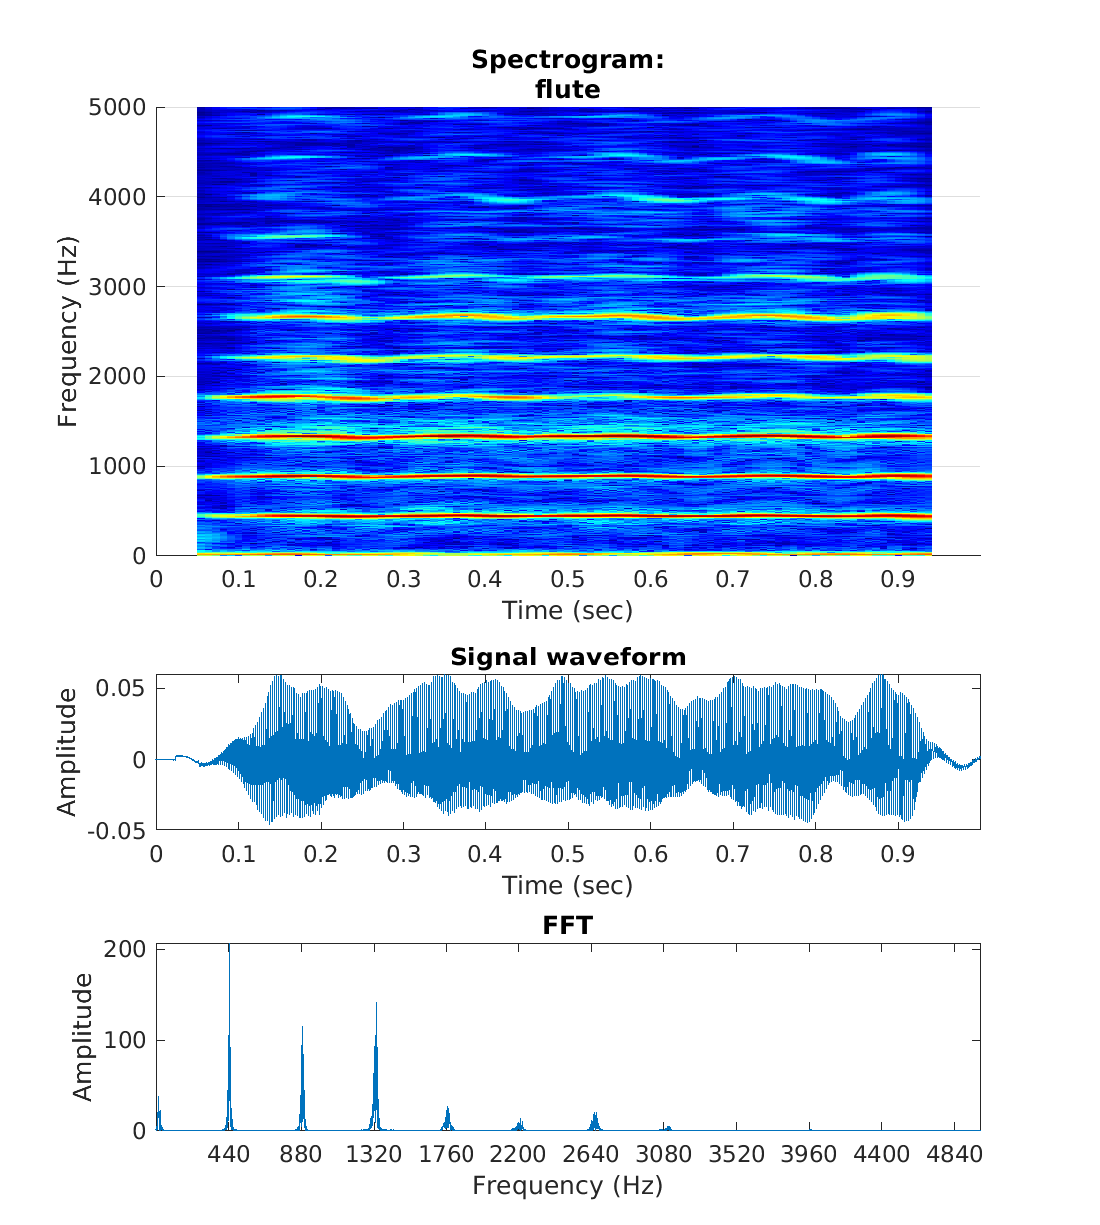
\includegraphics[width = .3\textwidth]{spectrogram_flute}
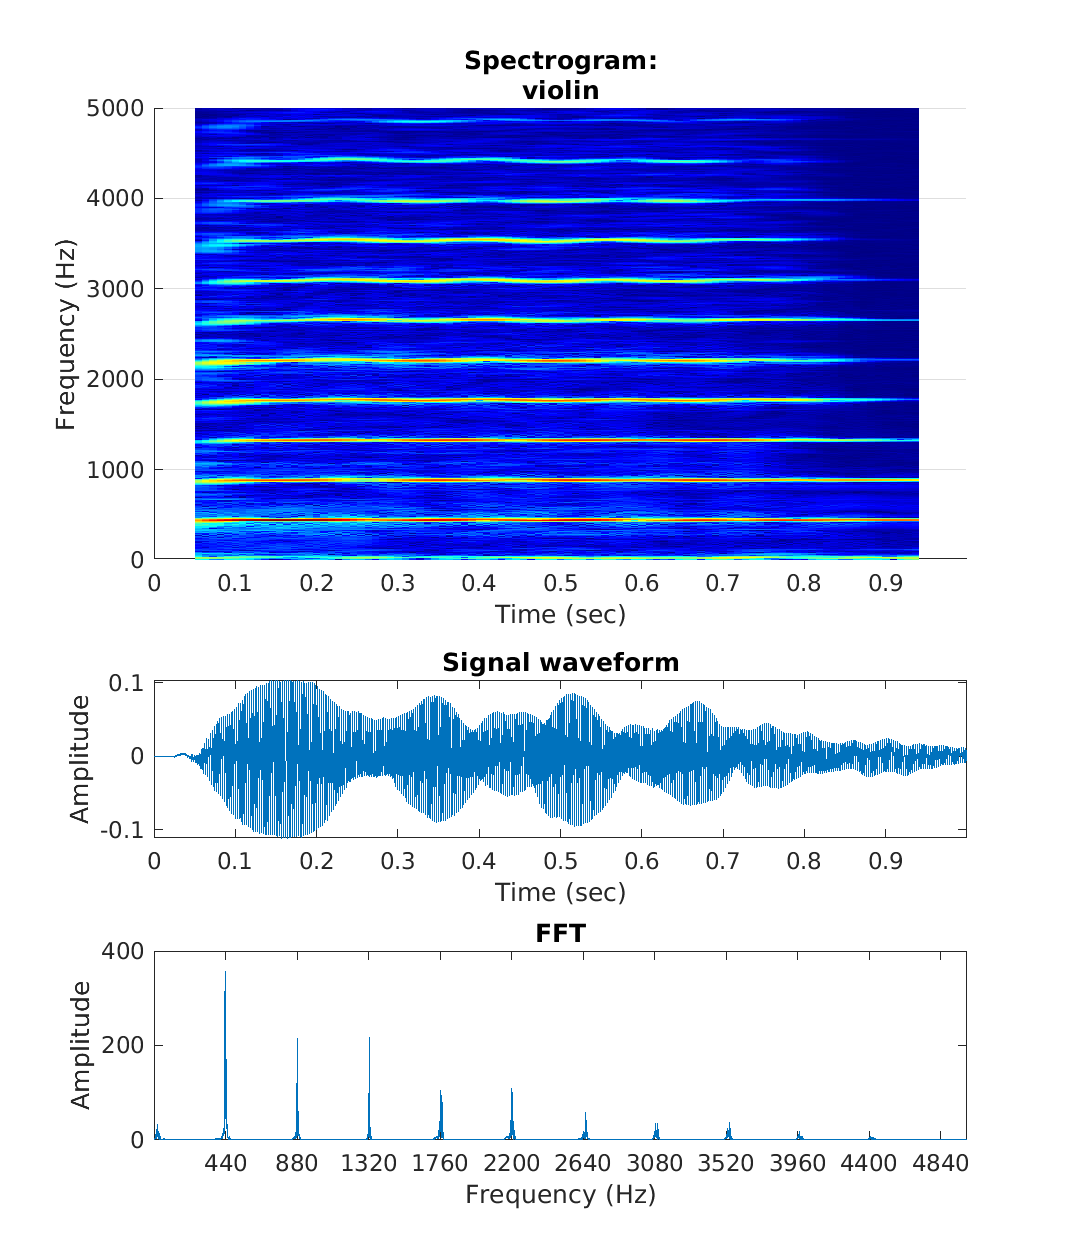
\includegraphics[width = .3\textwidth]{spectrogram_violin}\\
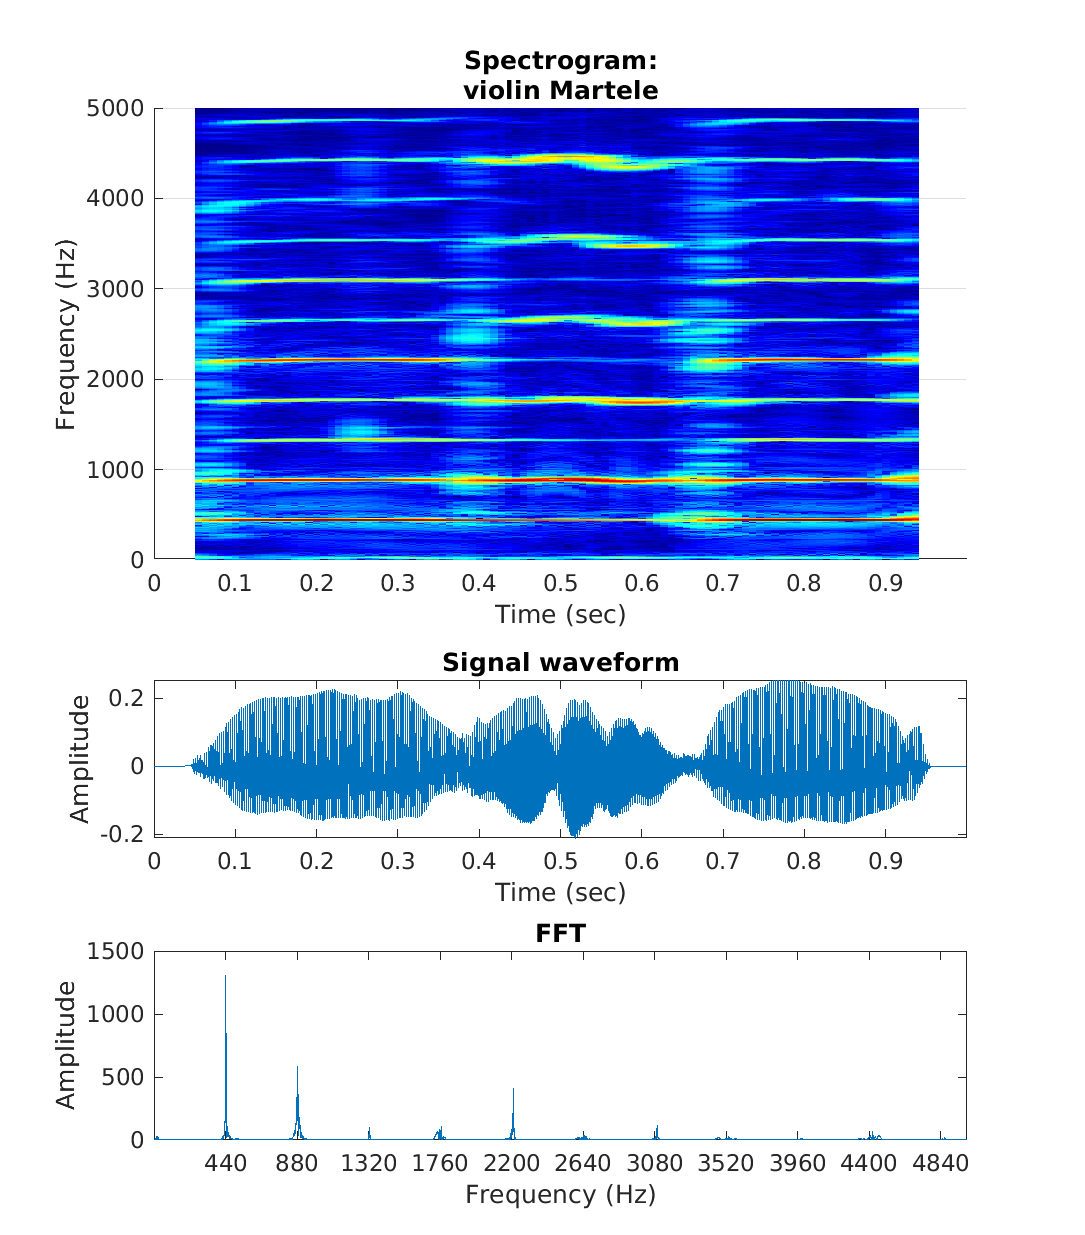
\includegraphics[width = .3\textwidth]{spectrogram_violin_phrase_forte_arco-martele}
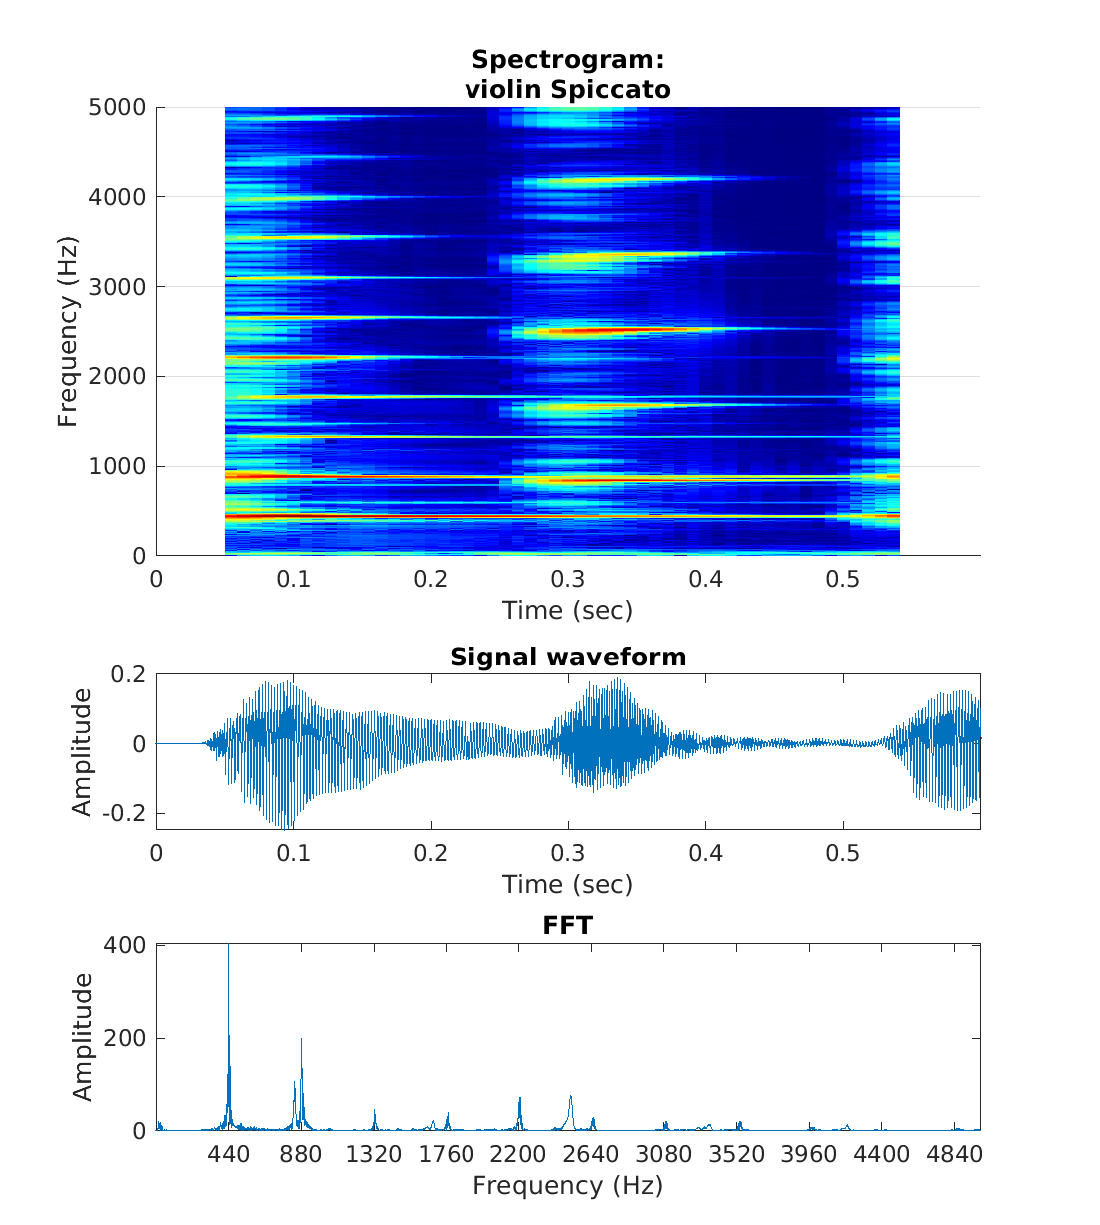
\includegraphics[width = .3\textwidth]{spectrogram_violin_phrase_forte_arco-spiccato}



\end{document}
